\chapter{Introduction}

Reversible computing initially gained interest as a way of avoiding the
fundamental energy requirement imposed by \emph{Landauer's Principle}.  It was
shown, initially in 1963 by Yves Lecerf\cite{lecerf63}, then again independently
by Charles Bennett\cite{Bennett:73} in 1973, that any classical irreversible
computation could be made reversible\footnotemark. Interest in reversible
computing has grown recently due to its applications to quantum computing.

\footnotetext{It is shown in both papers that a reversible Turing machine can
simulate an irreversible with some space overhead.}

In this thesis the focus will be on the compilation of reversible circuits in
the context of quantum computing. Tools for efficient circuit compilation are
necessary in the long term for implementing high level algorithms on a quantum
computer as well as in the short term for resource estimation.

Compiling an algorithm for a quantum computer is a multi-layered process.
Efficient implementations of operations are needed at the physical,
fault-tolerant and logical levels. An important part of compilation at the
logical level is the generation of reversible circuits. The goal of this thesis
is to describe a framework for the efficient compilation of high-level programs
into low level reversible circuits. It will discuss the use of pebble games for
circuit optimization. Also introduced is a new method for analysis in
reversible computation using a modified version of the reversible pebble game.


\section{Landauer's Principle}

Landauer's principle\cite{landauer61} states that any logically irreversible operation
must be accompanied by a corresponding entropy increase in non-information
bearing degrees of freedom. Another way to state this is that any operation
which does not preserve information must have an associated energy cost. This
can be understood through the second law of thermodynamics which states that
the entropy of a closed system cannot decrease. That is to say the number
of possible states a closed system might be in cannot decrease.

The minimum bound on the amount of energy required to perform an irreversible
operation is called the Landauer limit ($kT\ln 2$). Using reversible computing
it is in principle possible to avoid this cost by ensuring that no information
is lost in the computation.

%Currently the amount of energy expended on other inefficiencies is orders of
%magnitude higher then the energy loss due to Landauer's principle so this is
%not likely to be of practical use in the short term. As we approach these low
%energies it may become more relevant.

\section{Reversible Computation}

Normally when performing computations information is discarded. Actions such as
overwriting and clearing memory cause many states to be mapped to the same
state. So even if one had knowledge of the output operations involved in a computation it
may not be possible to recover the initial state. These types of computations
are therefore called irreversible.

A computation is called reversible if any state can be traced uniquely forwards
and backwards through time, or equivalently if each step in the computation is
bijective. Bennett\cite{Bennett:73} showed that in principle any computation
can be made reversible.

Reversible computing is relevant in the context of quantum computation since it
is necessary to be able to implement unitary operations\footnote{In the
classical domain unitary operations are equivalent to reversible operations.}.
Efficient generation of quantum circuits is important since in many quantum
algorithms the cost of implementing a reversible oracle dominates. For example
when Grover's algorithm is used to query a classical function the query must be
implemented as a reversible circuit. Since the diffusion operator is relatively
small compared to the size of many functions of interest\cite{gbm2016,sha2016}
achieving a small circuit size is very important.

The focus of this thesis is on efficiently generating the reversible parts of a
quantum computation using the circuit model. In a quantum computer conditional
operations require measurements to be made. The circuit model corresponds with
measurement free computation since all operations are applied unconditionally.
%\todo{mmosca: It's still interesting of course to execute
%circuits with intermediate measurements whose results we use to decide what to
%do next. Your focus is on implementing the reversible pieces}

In order for an operation to be considered reversible it must be forwards and
backward deterministic\footnote{In other words it must be bijective}. For example
Consider a classical computation where we have inputs $a$, and $b$ and wish to
know the output $a\land b$. The classical AND gate computes $(a,b)\mapsto
(a\land b)$, discarding the values of $a$ and $b$. Since this function is not
bijective (ex. $0\land 0 = 0$ and $1 \land 0 = 0$) it is not reversible.
Similarly the fanout gate $a\mapsto (a,a)$ is also not considered reversible.
This is because it is not backwards deterministic on all inputs; for example
given an input $(0,1)$ the reverse fanout gate has no defined output.

One way to make a reversible AND operation
is to instead use the bijective function $(a,b,c) \mapsto (a,b,a\land b \oplus
c)$. This is called the ``Toffoli Gate''.  (If $c$ is initialized to zero we
have $(a,b,0) \mapsto (a,b,a\land b)$).

Any irreversible function can be made reversible using the ``Bennett
Method''\cite{Bennett:73}. In this method each irreversible gate is replaced
with a reversible version with additional space allocated as necessary. Then
the final result is copied on to the newly allocated set of bits and the entire
circuit is repeated in reverse in order to uncompute any intermediate
information computed by the circuit(see \cref{fig:bennett}). So given an irreversible
function $f(x)$ (where $f(x)$ is of size $n$) we can use the Bennett method to
generate a reversible function $(x,0^{n+m}) \mapsto (x,f(x),0^m)$.

\begin{figure}
      \capstart
      \centering
      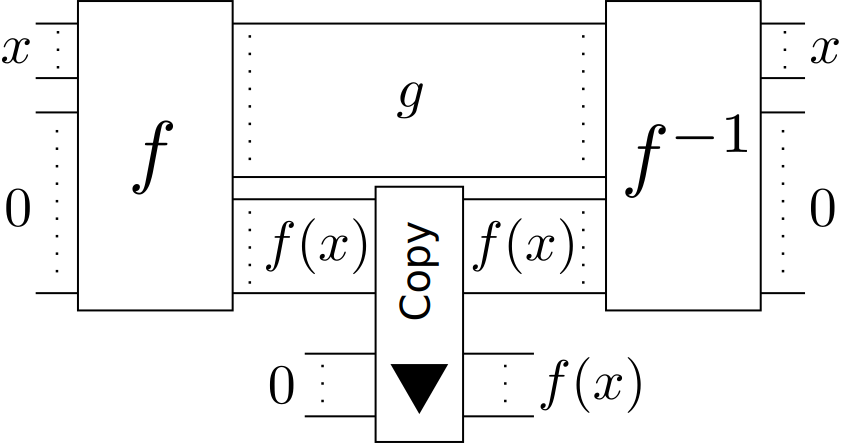
\includegraphics[width=0.8\hsize]{images/bennett}

      \caption{Bennett Method. Performs the operation
         $(x,0^n,0^m)\mapsto(x,f(x),0^m)$ where $n$ is the size of the output and $m$ is
         the number of ancilla needed for the computation of $f(x)$ Copy uses a cascade
         of CNot gates, i.e. it maps basis states:
         $(x_1,\dotsc,x_n,0^n)\mapsto(x_1,\dotsc,x_n,x_1,\dotsc,x_n)$. }

      \label{fig:bennett}
\end{figure}

The standard reversible gate set which will be used includes the following gates:

\begin{align*}
	&\text{Not:} a \mapsto \neg a \\
	&\text{Cnot:} (a,b) \mapsto (a,a\oplus b) \\
        &\text{Toffoli:} (a,b,c) \mapsto (a,b,ab\oplus c) \\
	&\text{Swap:} (a,b) \mapsto (b,a) \\
	&\text{Fredkin:} (a,b,c) \mapsto (a,\neg a b \oplus ac, ab\oplus \neg a c)
\end{align*}

Note another way of describing the Fredkin gate is as swap on $b$ and $c$
controlled on the value of $a$:

\begin{align*}
    (0,b,c) \mapsto (0,b,c)\\
    (1,b,c) \mapsto (1,c,b)
\end{align*}


\section{Quantum Circuits}

Analysis will be done using the Clifford plus T gate set.  This choice is made
due its availability in error correction schemes such as the surface
code\cite{fowler2012}.  Note that this gate set does not include the Toffoli
gate so it will have to be synthesised from more primitive gates in the set.
As shown in \cite{amy2013} this can be done using seven T-gates in T-depth 4.

Long range interactions are assumed to be inexpensive in this model compared to
the cost of T gates.

%\todo{Expand and mention the cost of state distillation as motivation}
%\todo {Show decomposition of Toffoli gate to Clifford+T and discuss what this
%means for circuit optimization.}
